\documentclass[letterpaper,12pt,fleqn]{article}
\usepackage{matharticle}
\usepackage{tikz}
\pagestyle{empty}
\newcommand{\T}{\mathscr{T}}
\newcommand{\B}{\mathcal{B}}
\renewcommand{\S}{\mathcal{S}}
\begin{document}
\section*{Order Topology}

\begin{definition}[Partial Ordering]
  Let \(X\) be a set and let \(\le\) be a binary operator on \(X\).  So say that \(\le\) is a \emph{partial ordering}
  on \(X\) means that for all \(x,y,z\in X\), \(\le\) is:
  \begin{description}
  \item[Reflexive:] \(x\le x\)
  \item[Antisymmetric:] \(x\le y\) and \(y\le x\implies x=y\)
  \item[Transitive:] \(x\le y\) and \(y\le z\implies x\le z\)
  \end{description}
  A set with such a partial ordering, denoted by \((X,\le)\), is called a \emph{poset}.
\end{definition}

\begin{definition}[Comparable]
  Let \((X,\le)\) be a poset.  To say that \(x,y\in X\) are \emph{comparable} means that \(x\le y\) or \(y\le \).
\end{definition}

\begin{example}[Subset]
  Let \(X\) be a set.  \(\subset\) is a partial ordering on \(2^X\), since some elements of \(2^X\) are not
  comparable.
\end{example}

\begin{notation}
  Let \((X,\le)\) be a poset and let \(a\in X\):
  \begin{gather*}
    a_{<}=\setb{x\in X}{x<a} \\
    a_{>}=\setb{x\in X}{x>a} \\
    (a,b)=\setb{x\in X}{a<x<b}=a_{>}\cap b_{<}
  \end{gather*}
\end{notation}

\begin{definition}[Total Ordering]
  Let \((X,\le)\) be a poset.  To say that \(\le\) is a \emph{total ordering} on \(X\) means that every
  \(x,y\in X\) is comparable.
\end{definition}

\begin{definition}[Order Topology]
  Let \((X,\le)\) be a total ordering and let:
  \[B=\setb{a_{<}}{a\in X}\cup\setb{a_{>}}{a\in X}\cup\setb{(a,b)}{a,b\in X}\]
  \(B\) is a basis for a topology \(\T\) on \(X\) called the \emph{order} topology.
\end{definition}

\begin{definition}[Lexicographic Order]
  Let \(A,\le_A\) and \(B,\le_B\) be totally orderings.  The \emph{lexicographic} or \emph{dictionary} ordering on
  \(A\times B\) is given by:
  \[(a_1,b_1)<(a_2,b_2)\iff a_1<a_2\ \text{or}\ a_1=a_2\ \text{and}\ b_1<b_2\]
\end{definition}

\begin{definition}[Lexicographically Ordered Square]
  The square \([0,1]\times[0,1]\) with the lexicographic order and its associated order topology is called the
  \emph{lexicographically ordered square}.
\end{definition}

\begin{example}
  Draw pictures of various open sets in the lexicographically ordered square.

  \begin{minipage}{2in}
    \centering
    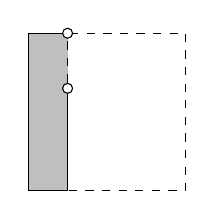
\begin{tikzpicture}
      \draw [dashed] (0,0) rectangle (2,2);
      \fill [lightgray] (0,0) rectangle (0.5,2);
      \node (a) [draw,circle,inner sep=0in,minimum size=0.05in,fill=white] at (0.5,1.3) {};
      \node (b) [draw,circle,inner sep=0in,minimum size=0.05in,fill=white] at (0.5,2) {};
      \draw (b) -- (0,2) -- (0,0) -- (0.5,0) -- (a);
      \draw [dashed] (a) -- (b);
    \end{tikzpicture}

    \(a_{<}\)
  \end{minipage}
  \begin{minipage}{2in}
    \centering
    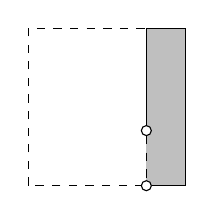
\begin{tikzpicture}
      \draw [dashed] (0,0) rectangle (2,2);
      \fill [lightgray] (1.5,0) rectangle (2,2);
      \node (a) [draw,circle,inner sep=0in,minimum size=0.05in,fill=white] at (1.5,0.7) {};
      \node (b) [draw,circle,inner sep=0in,minimum size=0.05in,fill=white] at (1.5,0) {};
      \draw (a) -- (1.5,2) -- (2,2) -- (2,0) -- (b);
      \draw [dashed] (a) -- (b);
    \end{tikzpicture}

    \(a_{>}\)
  \end{minipage}
  \begin{minipage}{2in}
    \centering
    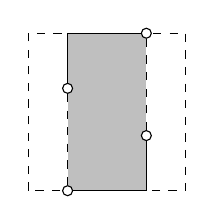
\begin{tikzpicture}
      \draw [dashed] (0,0) rectangle (2,2);
      \fill [lightgray] (0.5,0) rectangle (1.5,2);
      \node (a) [draw,circle,inner sep=0in,minimum size=0.05in,fill=white] at (0.5,1.3) {};
      \node (b) [draw,circle,inner sep=0in,minimum size=0.05in,fill=white] at (1.5,0.7) {};
      \node (c) [draw,circle,inner sep=0in,minimum size=0.05in,fill=white] at (0.5,0) {};
      \node (d) [draw,circle,inner sep=0in,minimum size=0.05in,fill=white] at (1.5,2) {};
      \draw (a) -- (0.5,2) -- (d);
      \draw (b) -- (1.5,0) -- (c);
      \draw [dashed] (a) -- (c);
      \draw [dashed] (b) -- (d);
    \end{tikzpicture}

    \((a,b)\)
  \end{minipage}
\end{example}

\begin{example}
  Let \(\S\) be the lexicographically ordered square and \(A=\setb{\left(\frac{1}{n},0\right)}{n\in\N}\subset\S\).
  Determine the closure of \(A\).

  \(\bar{A}=A\cup\setb{(0,y)}{y\in[0,1]}\)
\end{example}

\end{document}
